\section{eo\-PBILAdditive$<$ EOT $>$ Class Template Reference}
\label{classeo_p_b_i_l_additive}\index{eoPBILAdditive@{eoPBILAdditive}}
Distribution Class for PBIL algorithm (Population-Based Incremental Learning, Baluja and Caruana 96).  


{\tt \#include $<$eo\-PBILAdditive.h$>$}

Inheritance diagram for eo\-PBILAdditive$<$ EOT $>$::\begin{figure}[H]
\begin{center}
\leavevmode
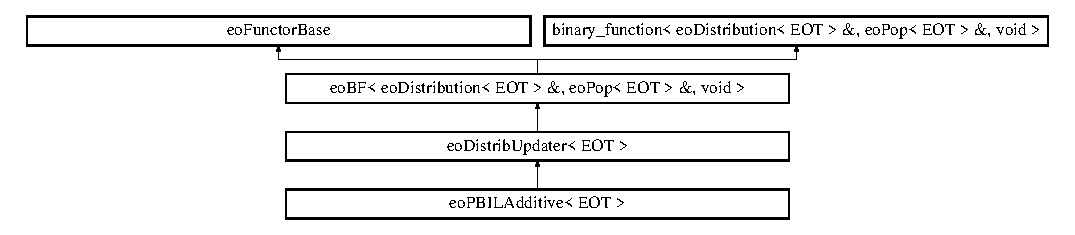
\includegraphics[height=2.71186cm]{classeo_p_b_i_l_additive}
\end{center}
\end{figure}
\subsection*{Public Member Functions}
\begin{CompactItemize}
\item 
{\bf eo\-PBILAdditive} (double \_\-LRBest, unsigned \_\-nb\-Best=1, double \_\-tolerance=0.0, double \_\-LRWorst=0.0, unsigned \_\-nb\-Worst=0)\label{classeo_p_b_i_l_additive_a0}

\begin{CompactList}\small\item\em Ctor with parameters using the default values is equivalent to using {\bf eo\-PBILOrg}{\rm (p.\,\pageref{classeo_p_b_i_l_org})}. \item\end{CompactList}\item 
virtual void {\bf operator()} ({\bf eo\-Distribution}$<$ {\bf EOT} $>$ \&\_\-distrib, {\bf eo\-Pop}$<$ {\bf EOT} $>$ \&\_\-pop)\label{classeo_p_b_i_l_additive_a1}

\begin{CompactList}\small\item\em Update the distribution from the current population. \item\end{CompactList}\end{CompactItemize}
\subsection*{Private Attributes}
\begin{CompactItemize}
\item 
double {\bf max\-Bound}\label{classeo_p_b_i_l_additive_r0}

\item 
double {\bf min\-Bound}\label{classeo_p_b_i_l_additive_r1}

\item 
double {\bf LR}\label{classeo_p_b_i_l_additive_r2}

\item 
unsigned {\bf nb\-Best}\label{classeo_p_b_i_l_additive_r3}

\item 
unsigned {\bf nb\-Worst}\label{classeo_p_b_i_l_additive_r4}

\item 
double {\bf lrb}\label{classeo_p_b_i_l_additive_r5}

\item 
double {\bf lrw}\label{classeo_p_b_i_l_additive_r6}

\end{CompactItemize}


\subsection{Detailed Description}
\subsubsection*{template$<$class EOT$>$ class eo\-PBILAdditive$<$ EOT $>$}

Distribution Class for PBIL algorithm (Population-Based Incremental Learning, Baluja and Caruana 96). 

This class implements an extended update rule: in the original paper, the authors used

p(i)(t+1) = (1-LR)$\ast$p(i)(t) + LR$\ast$best(i)

here the same formula is applied, with some of the best individuals and for some of the worst individuals (with different learning rates) 



Definition at line 46 of file eo\-PBILAdditive.h.

The documentation for this class was generated from the following file:\begin{CompactItemize}
\item 
eo\-PBILAdditive.h\end{CompactItemize}
